%-----------------------------------------------------------------------
% 
%-----------------------------------------------------------------------
%
%     
%
%
%%%%%%%%%%%%%%%%%%%%%%%%%%%%%%%%%%%%%%%%%%%%%%%%%%%%%%%%%%%%%%%%%%%%%%%%


\documentclass[twoside]{article}
\usepackage{amsmath,amsthm,amssymb,verbatim}

%     If your article includes graphics, uncomment this command.
\usepackage{graphicx}

%     If the article includes commutative diagrams, ...
%\usepackage[cmtip,all]{xy}

\usepackage{url}

\usepackage{fancyhdr}
\pagestyle{fancy}

\def\blfootnote{\xdef\@thefnmark{}\@footnotetext} 
\long\def\symbolfootnote[#1]#2{\begingroup%
\def\thefootnote{\fnsymbol{footnote}}\footnote[#1]{#2}\endgroup} 

	\addtolength{\oddsidemargin}{1cm}
	\addtolength{\evensidemargin}{-1cm}

\setcounter{page}{1}

\begin{document}

%     If you need symbols beyond the basic set, uncomment this command.
%\usepackage{amssymb}


\newtheorem{theorem}{Theorem}[section]
\newtheorem{lemma}[theorem]{Lemma}

\theoremstyle{definition}
\newtheorem{definition}[theorem]{Definition}
\newtheorem{example}[theorem]{Example}
\newtheorem{xca}[theorem]{Exercise}

\theoremstyle{remark}
\newtheorem{remark}[theorem]{Remark}

\numberwithin{equation}{section}


\date{}
\lhead[]{}
\chead[\underline{Deep Learning for Riemann Zeta}]{\it{O. Shanker}}
\rhead[]{}

% \title[short text for running head]{full title}
\title{\bf{Deep Learning for Riemann Zeta Function: Large Values and Karatsuba problem}}

\maketitle


%    author one information
% \author[short version for running head]{name for top of paper}
\author{{\textbf{O. Shanker}},}
\thanks{ Mountain View, CA 94041, U. S. A. email: oshanker@gmail.com}

\thispagestyle{fancy}

%    Abstract is required.
\begin{abstract}
We present a new hitherto unknown symmetry in the value
distribution of the characteristic polynomial of the Circular Unitary Ensemble (CUE)
 at discrete points. This is significant because the symmetry properties
are fundamental aspects of a system. We show that the value distribution 
can be expressed in terms of three functions 
which do not depend on the angle characterizing the Generalized Gram point.
These relationships are very similar to those  observed for 
the Riemann zeta function.
\end{abstract}
{\textbf {Keywords}:} Circular Unitary Ensemble, Riemann zeta, Value Distribution, Symmetry 
{\textbf {Mathematics Subject Classification (MSC)}:} 11M06, 11-04.


\symbolfootnote[0]{*}


\section{Introduction}

Karatsuba problem.  Many applications of machine learning in mathematics.

RMT has found applications~\cite{KeatingSnaith 2000,Odlyzko 1992} 
in many areas of physics, mathematics,  probability, statistics, and engineering. 
 RMT is closely associated with the study of the zeroes of the Riemann zeta function 
 and Generalized Zeta functions. The zeros are of interest to mathematicians and physicists. 
Mathematicians 
study the spacings because of its applications to analytic number theory, 
while physicists study it because of its  relation 
to the theory of the spectra of random matrix theories 
and the spectra of classically chaotic quantum systems.
Ref.~\cite{Chhaibi 2014} shows that the characteristic polynomial 
of the CUE has a limiting form when properly rescaled. 
See Ref.~\cite{Francesco 2007,os6, Hanga 2020} for  further references,
examples and discussion. 
 Ref.~\cite{KeatingSnaith 2000} shows that the CUE provides
a good model for the moments and other properties of the $|\zeta(1/2 + it)|$.

We were motivated to do the current study because of almost identical 
properties observed
for the Riemann zeta function and Dirichlet $L$ functions. 
Ref.~\cite{Shanker 2018a,Shanker 2018b} studied 
the distribution of $Z(t)$ values 
at Gram points and showed  that  the  value
distribution of the Hardy $Z$ function at discrete points is anti-symmetrical for 
reflections around the mid-points of the Gram intervals (Eq.~\ref{eq:Rieantisym}) 
and symmetrical for reflections around the Gram points(Eq.~\ref{eq:Riesym}). 
Ref.~\cite{Shanker 2020} showed that the value distribution of the Riemann zeta function 
can be expressed in terms of three  functions 
 which do not depend on the angle characterizing the Generalized Gram point. 

\section{\label{sec2}Materials and Methods}

\subsection{\label{seckaratsuba}Karatsuba Problem}


\subsection{\label{secwhy}Why Machine Learning?}

At large heights evaluating the Riemann zeta function  is a non-trivial task, requiring much computer time 
(and some knowledge of special techniques to find the roots).  It would be useful to apply
machine learning
as a guide to identify the T values where we can expect to see the behaviour of interest.
Ref~\cite{osneural} found that the behavior of the zeta function at Gram points 
is a good starting point to extract features for use in prediction. 
Ref.~\cite{Shanker 2018a} further showed that Gram points have interesting properties 
which distinguish them from random points on the critical line, supports the conclusion. 


It is known (Ref.~\cite{Shanker 2018b}) that the average value of the 
$Z$ distribution is $2cos(\phi)$ where $\phi$
is the angle characterizing the Generalized Gram point. We have also shown
(Ref.~\cite{Shanker 2020}) that the probability distributions
satisfy the anti-symmetry relation 
\begin{equation}
p_{\phi}(z) = p_{\phi+\pi}(-z)
\label{eq:Rieantisym}
\end{equation}
and the symmetry relation is
\begin{equation}
p_{\phi}(z) = p_{2\pi-\phi}(z).
\label{eq:Riesym}
\end{equation}
Ref.~\cite{Shanker 2020} showed 
that the probability distributions at different $\phi$ can all be expressed in
terms of three functions which are independent of $\phi$ and depend only on $z$.
These are the observations which we wanted to model using the CUE. For generating the
CUE samples for the study we extend the programs and results of Ref.~\cite{Francesco 2007}.

\begin{figure*}
\centering
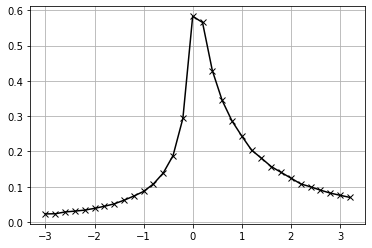
\includegraphics[width=0.8\textwidth]{1.png}
\caption[]{ 
  Probability density  for $\phi = 0$. 
  }
\vspace{1mm}
\label{z1}
\end{figure*}

\begin{figure*}
\centering
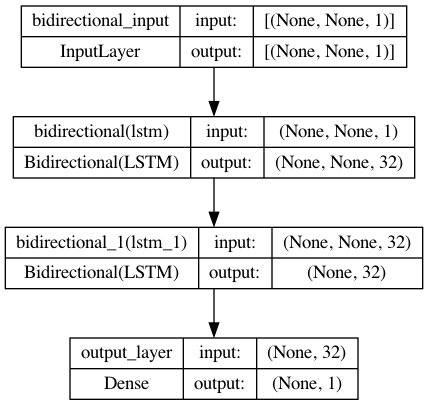
\includegraphics[width=0.8\textwidth]{2.png}
\caption[]{ 
  Probability density  for $\phi = \pi/2$. 
  }
\vspace{1mm}
\label{z2}
\end{figure*}

\begin{figure*}
\centering
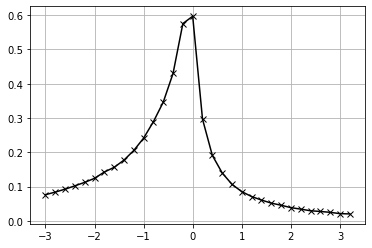
\includegraphics[width=0.8\textwidth]{3.png}
\caption[]{ 
  Probability density  for $\phi = \pi$. Compare with
 Fig.~\ref{z1} to observe the mirror symmetry.
  }
\vspace{1mm}
\label{z3}
\end{figure*}

\begin{figure*}
\centering
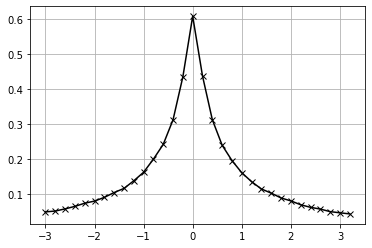
\includegraphics[width=0.8\textwidth]{4.png}
\caption[]{ 
  Probability density  for $\phi = 3\pi/2$. 
  }
\vspace{1mm}
\label{z4}
\end{figure*}



\section{\label{sec3}Results}

\subsection{\label{sec3.1} Choosing the Model}

Since the Riemann zeta studies were done at a
height $T = 10^{12}$, we use the well-known correspondence $N \thicksim \ln(T/2\pi)$ where $N$ 
is the size of the unitary matrix we should consider. Thus, we chose $N = 26$ for our
study.  We studied $10000$ sample $U$ to generate the distributions.

The characteristic polynomial can be written as
\begin{align}
\Lambda(U, \theta) = det(I-U\exp^{-i\theta})\\
                   = \prod_{n}(1-\exp^{i(\theta_{n} - \theta)}).
\label{eq:cueDet}
\end{align}
This expression simplifies to
\begin{align}
\Lambda(U, \theta)  = 2^N\exp^{i(3N\pi/2 + \sum_{n}\theta_{n}/2 - N\theta/2)}\prod_{n}\sin((\theta_{n} - \theta)/2).
\label{eq:cueExpanded}
\end{align}
In analogy with the $Z$ in the Riemann zeta case, we can identify a $Z_{CUE}$ by defining
\begin{align}
Z_{CUE}(\theta))    = \exp^{-i(3N\pi/2 + \sum_{n}\theta_{n}/2 - N\theta/2)}\Lambda(U, \theta)\\
                    = 2^N\prod_{n}\sin((\theta_{n} - \theta)/2).
\label{eq:cueZ}
\end{align}
$Z_{CUE}(\theta))$ is real valued,
and we have $|Z_{CUE}(\theta)| = |\Lambda(U, \theta)|$. The analogue of the Riemann zeta 
Gram points occurs when $\Lambda(U, \theta)$ is real, i.e., 
$(3N\pi/2 + \sum_{n}\theta_{n}/2 - N\theta/2) = m\pi$.
We call $\theta$  a CUE generalized Gram point with value $\phi$  if
$(3N\pi/2 + \sum_{n}\theta_{n}/2 - N\theta/2) = 2k\pi + \phi$, where $0 \le \phi < 2\pi$.
For a given $\phi$, we have $N$ distinct CUE generalized Gram points spaced uniformly
around the unit circle.
The definition for the probability distribution is analogous to the Riemann zeta definition.

The CUE probability distributions satisfy (see Fig.~\ref{z1},~\ref{z2},~\ref{z3},~\ref{z4}) 
the anti-symmetry relation 
\begin{equation}
p_{\phi}(z) = p_{\phi+\pi}(-z)
\label{eq:antisym}
\end{equation}
and the symmetry relation 
\begin{equation}
p_{\phi}(z) = p_{2\pi-\phi}(z).
\label{eq:sym}
\end{equation}
We also found  (see Table~\ref{tab:mean12}) that the average value of the 
distribution is $2cos(\phi)$ where $\phi$
is the angle characterizing the CUE generalized Gram point, i.e., 
\begin{equation}
<z>_{\phi} = 2\cos(\phi).
\label{eq:cosphi}
\end{equation}
Thus, we reproduce the behaviour 
for the Riemann zeta case.


\begin{table}
\centering \(\begin{array}{cccccccccccc}

\hline
0     &\pi/2  &\pi  &3\pi/2  \\
2.03  &0.00  &-2.02 & -0.03  \\
\hline
\end{array}\)
\caption{Mean  $Z(t)$. Row 1: $\phi$, 
Row 2: mean~$Z$}
\label{tab:mean12}
\end{table}


\begin{figure*}
\centering
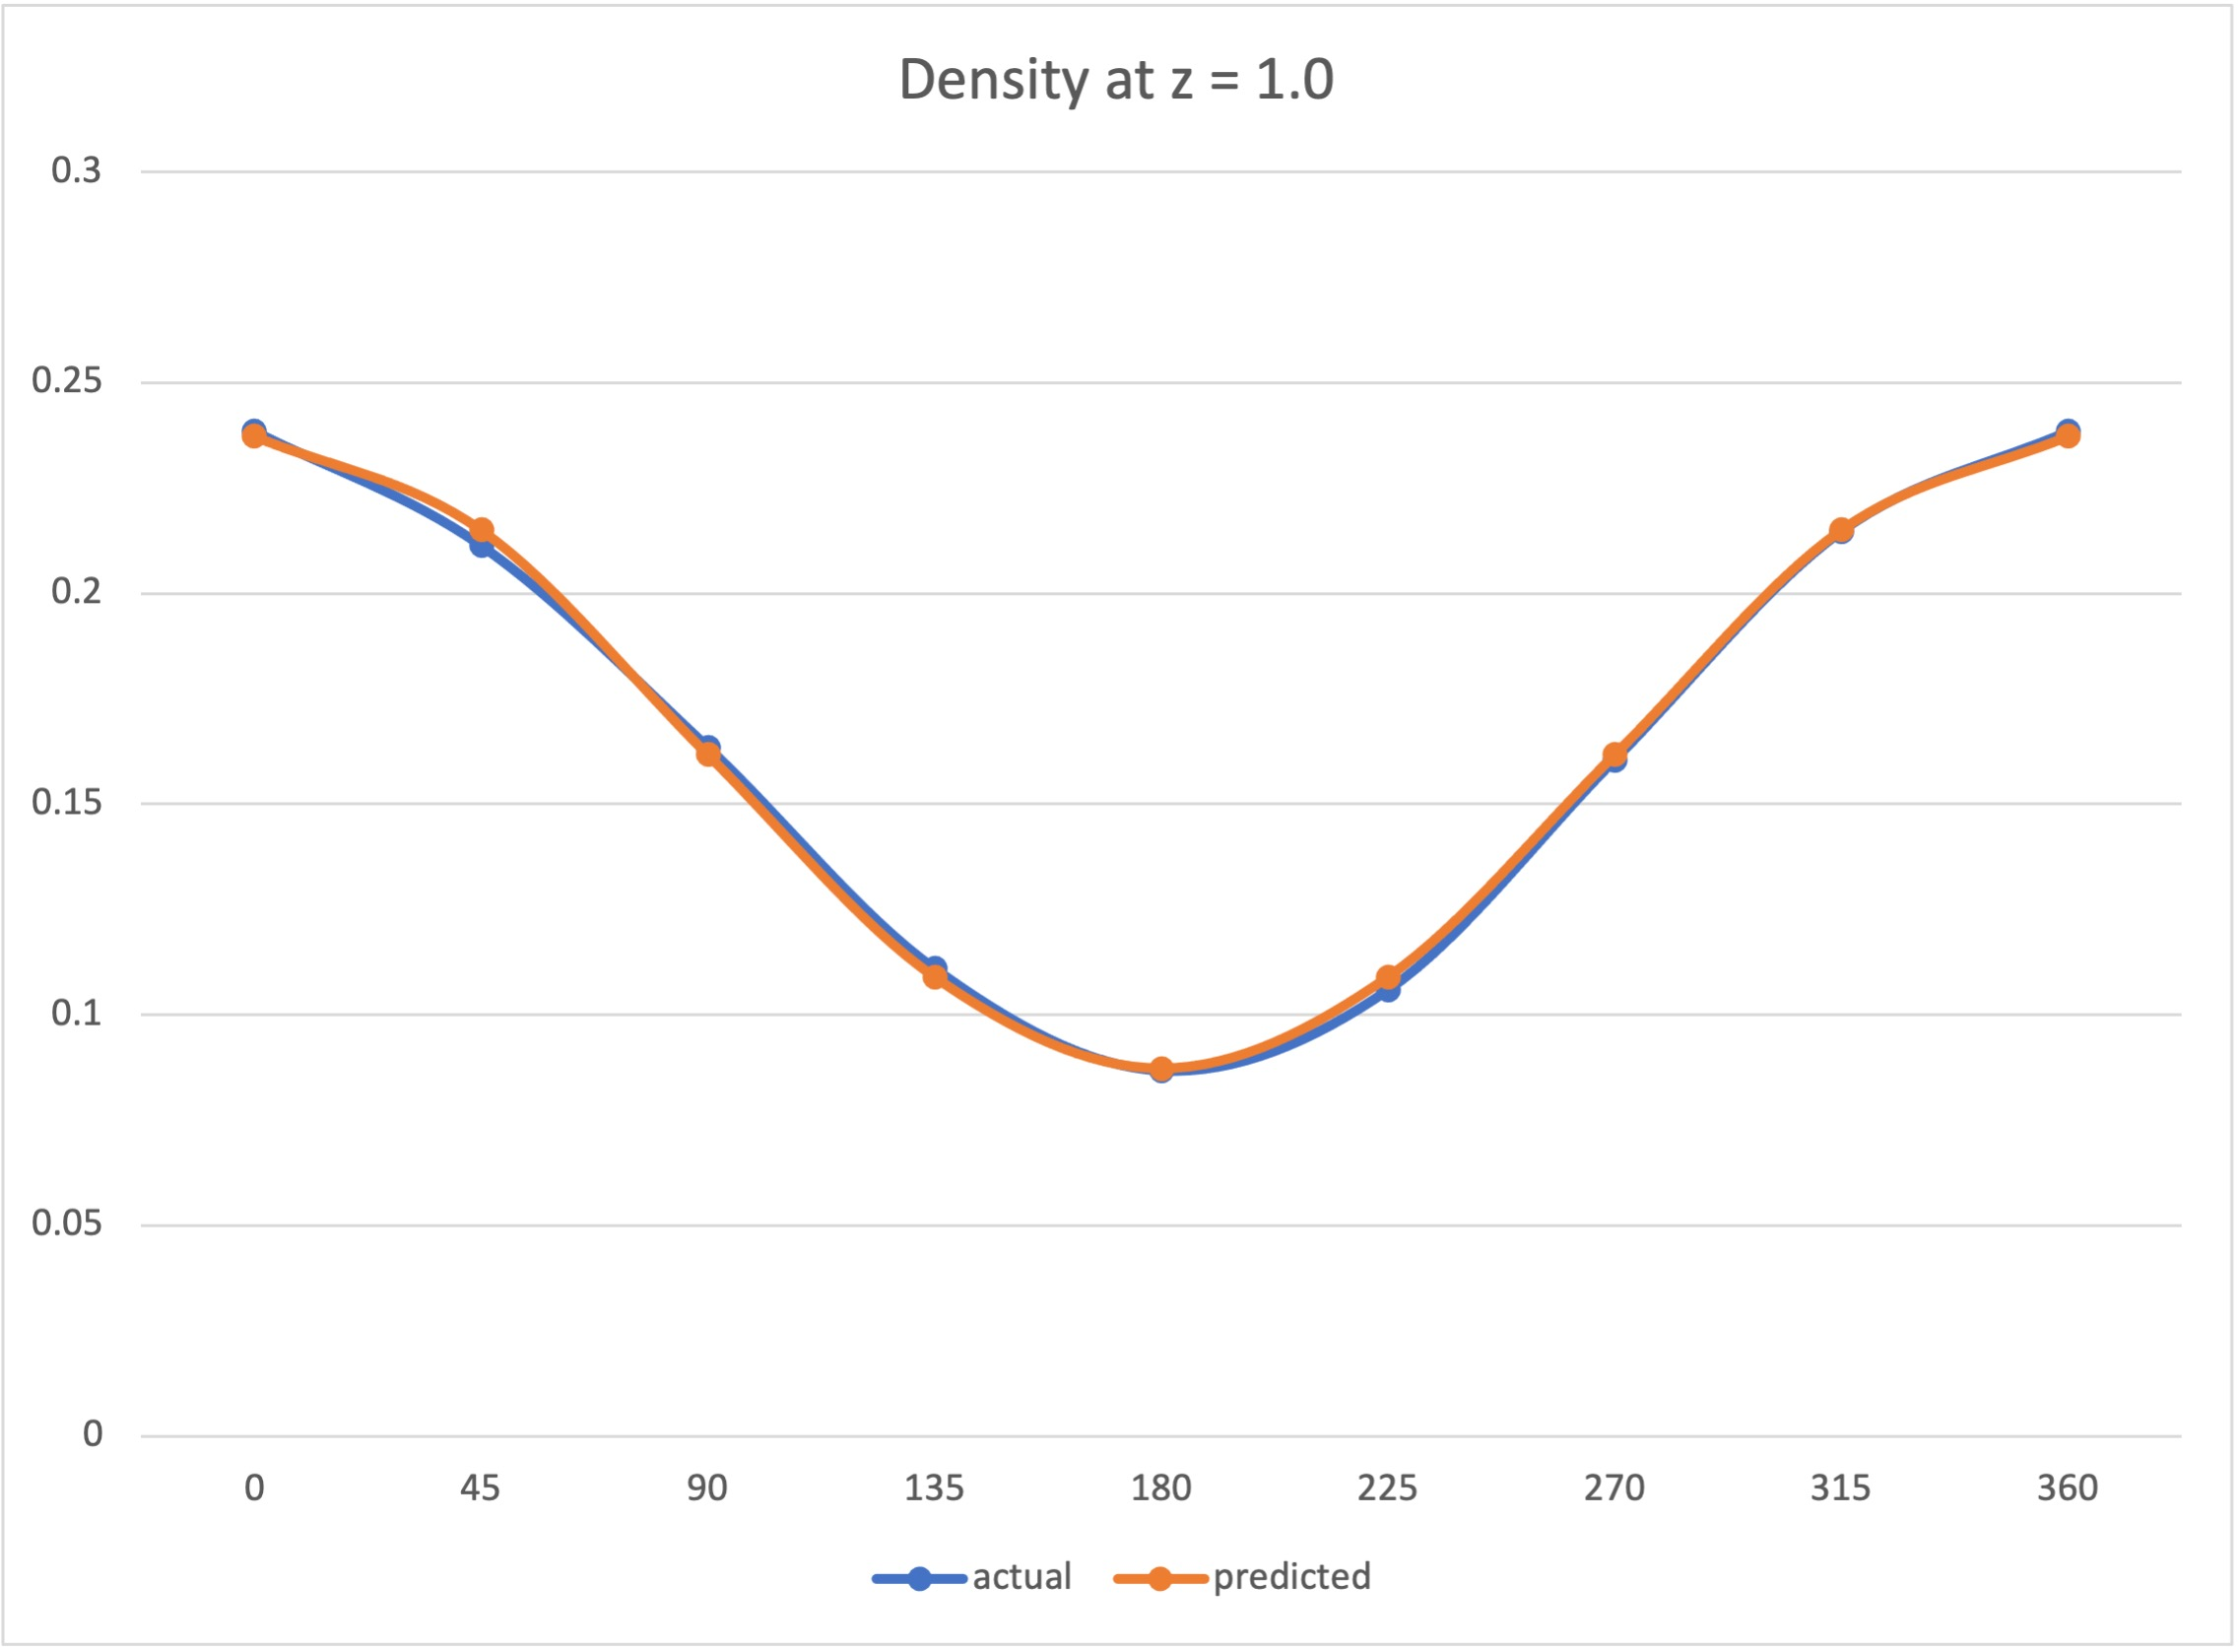
\includegraphics[width=0.8\textwidth]{z1.jpg}
\caption[]{ 
 Test of universality. Comparison of probability density prediction from
 universality with actual values, for $z=1.0$. The y axis is the probability density.
 The x axis is the angle characterizing the Generalized Gram point.
  }
\vspace{1mm}
\label{z05}
\end{figure*}

\begin{figure*}
\centering
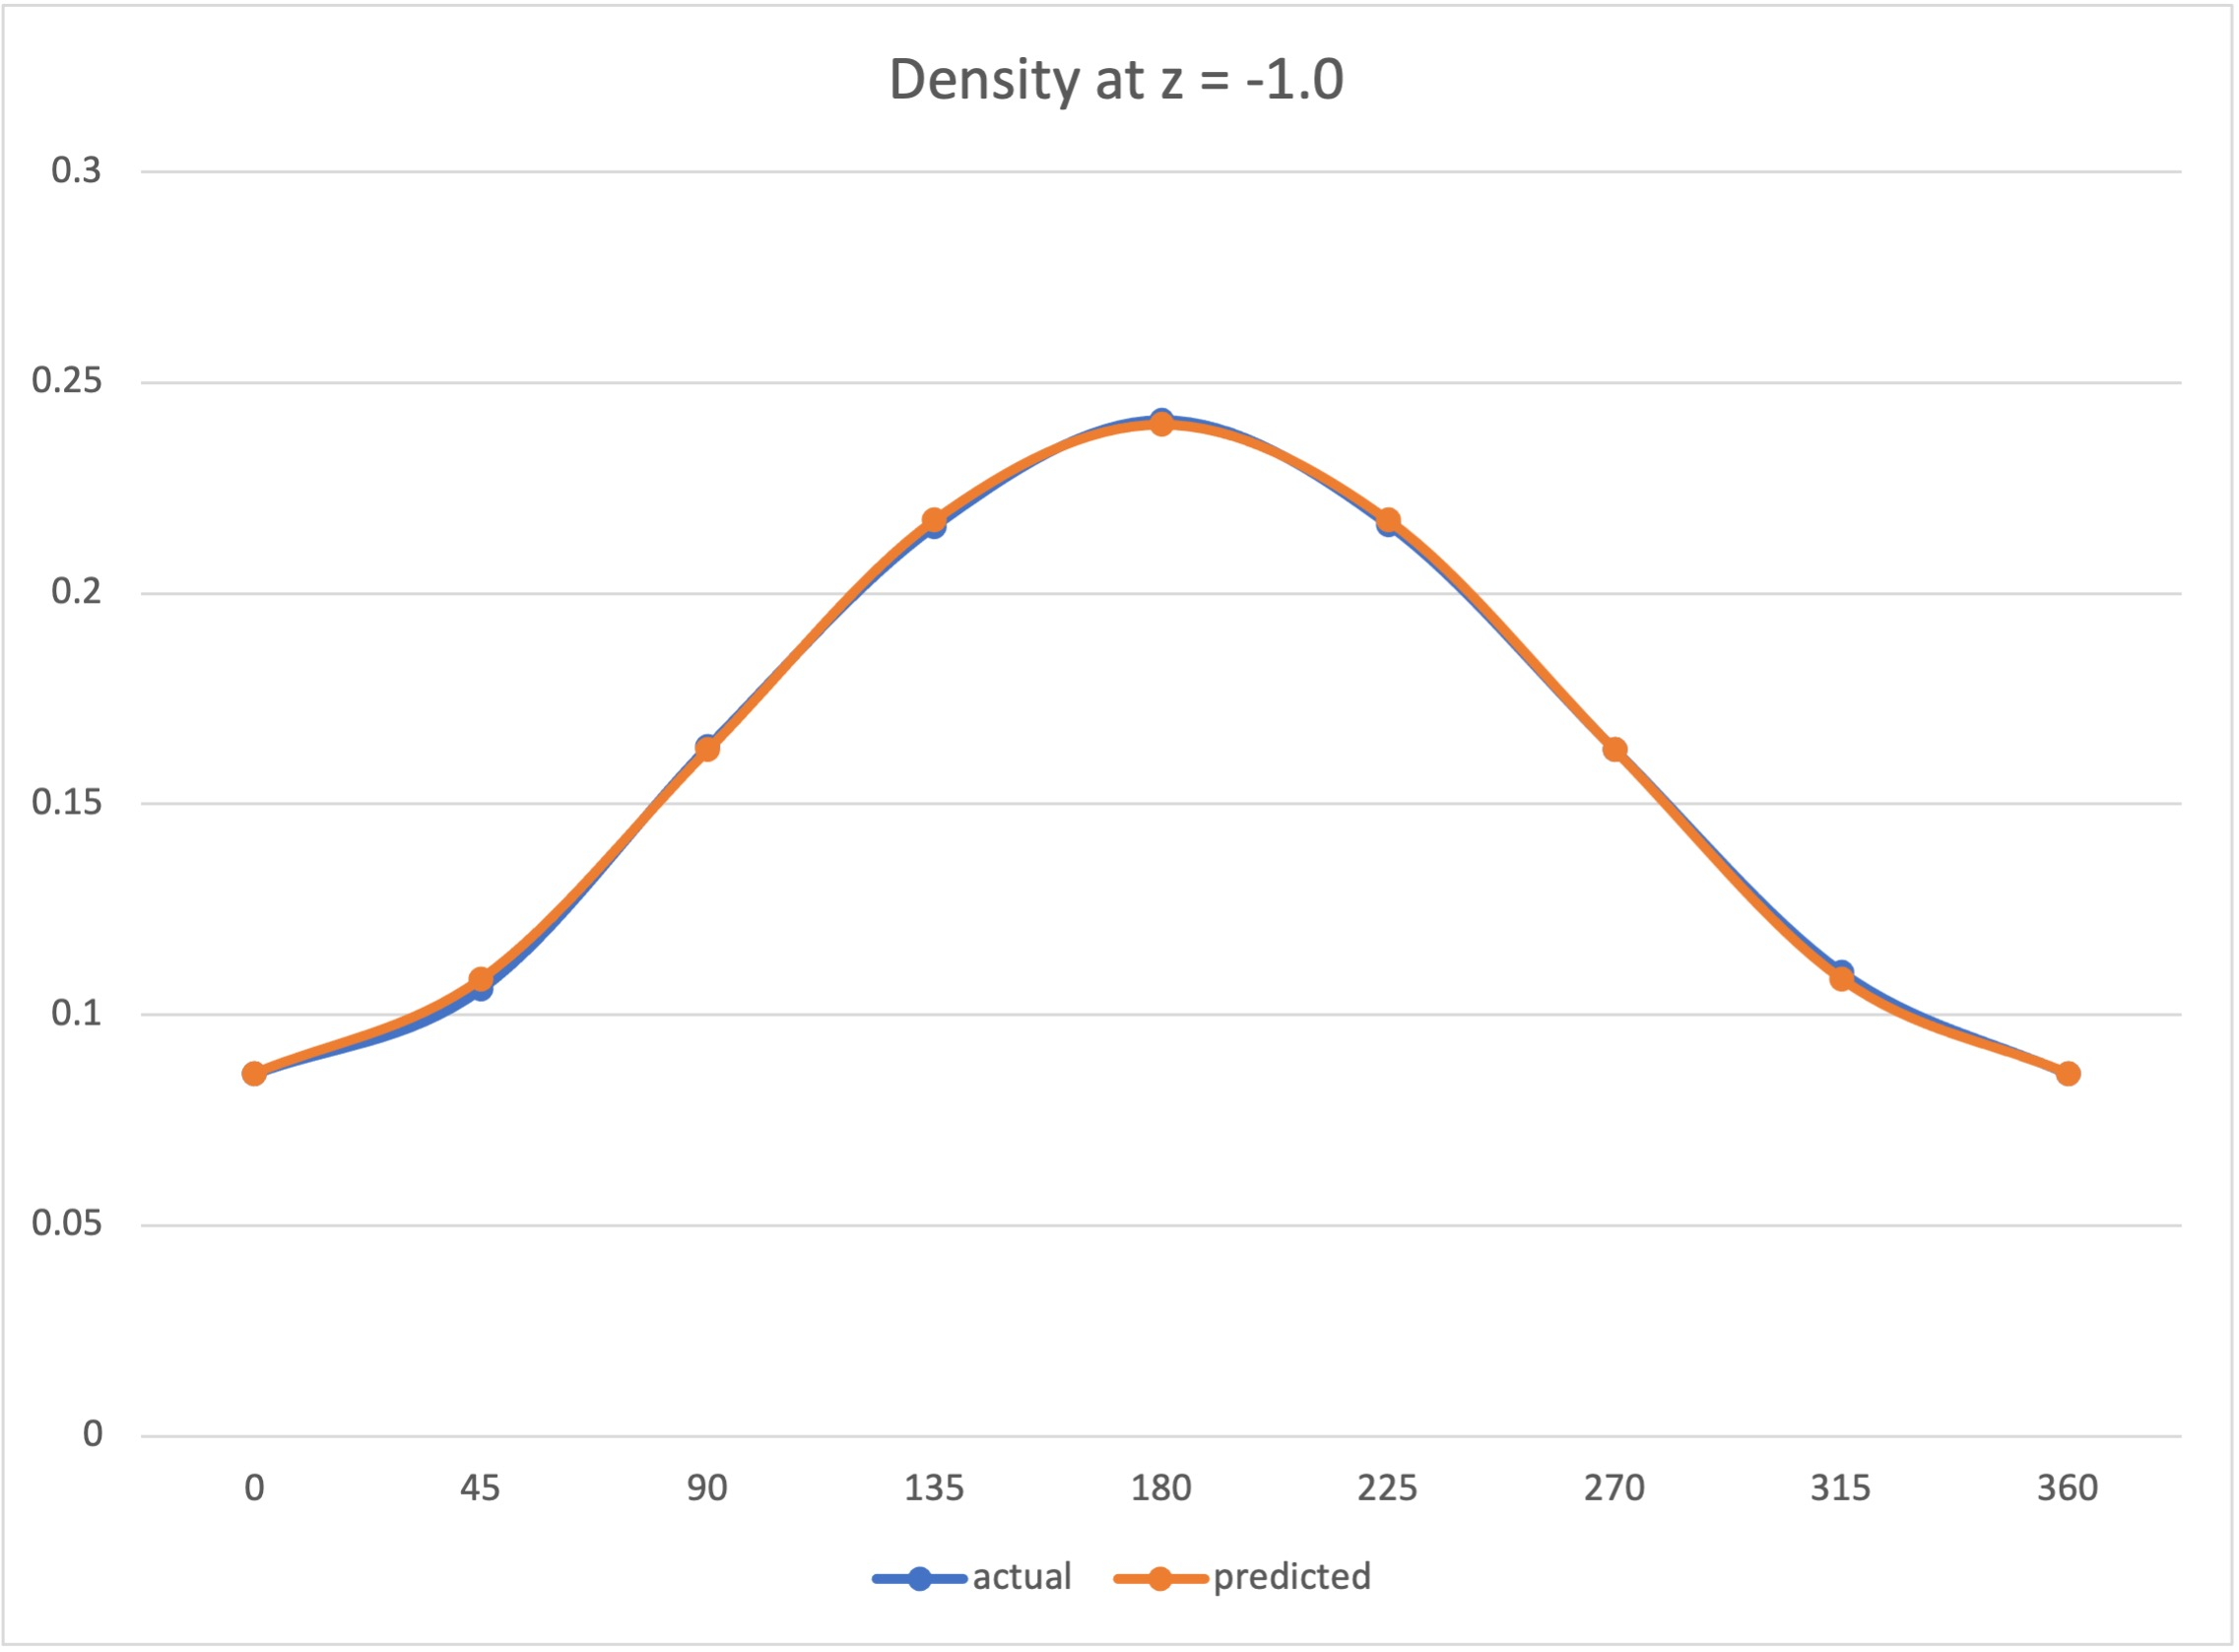
\includegraphics[width=0.8\textwidth]{z_1.jpg}
\caption[]{ 
 Test of universality. Comparison of probability density prediction from
 universality with actual values, for $z=-1.0$. 
  }
\vspace{1mm}
\label{z00}
\end{figure*}

\subsection{\label{relation}Training,  Model predictions}

For the Riemann zeta probability distributions, we found~\cite{Shanker 2020}
that the probability distributions at different $\phi$ can all be expressed in
terms of three functions which are independent of $\phi$ and depend only on $z$.
We show that such a relation holds for the CUE distributions also.
This is a very intriguing direction to probe more deeply.

The universality relation is
\begin{equation}
p_{\phi}(z) = A(z) + B(z)\cos(\phi) +C(z)\cos(2\phi),
\label{eq:universality}
\end{equation}
where $A(z)$, $B(z)$ and $C(z)$ are  functions which do not depend on $\phi$. 
We estimated $A(z)$, $B(z)$ and $C(z)$ by fitting Eq.~\ref{eq:universality} to the actual
probability densities for several values of $z$ and $\phi$. 
Fig~\ref{z05} and Fig.~\ref{z00} show the comparison of the predictions 
from the universality 
relation to the actual probability densities, for some values of the argument $z$.
We find that the function 
$B(z)$ is anti-symmetric in $z$, and $A(z)$ and $C(z)$ are symmetric in $z$, which 
leads to Eq.~\ref{eq:sym} and Eq.~\ref{eq:antisym}.
The figures show the excellent agreement of the actual probability densities with the
universality relations prediction.


\section{\label{conclusions}Conclusions}

We discovered new anti-symmetry and symmetry properties 
for the value distribution of the CUE characteristic polynomial at discrete points. 
We presented a simple relation for the average value 
of the  distribution. We showed that the value distribution 
can be expressed in terms of three  functions 
 which do not depend on the angle characterizing the Generalized Gram point. 
These relations are very similar to the relations observed for 
the Riemann zeta function.

\section*{Acknowledgments and Funding Statement}

 The study was done as an independent researcher. There was no
external funding.

\section*{Ethical Compliance}

 No procedures were performed  involving human participants in the study.

\section*{Data Availability Statement}

The computer programs used during the current study are
available from the corresponding author on reasonable request.

\section*{Conflict of Interest declaration} 

The authors declare that they have no affiliations with or involvement in any organization 
or entity with any financial interest in the subject matter or materials discussed 
in this manuscript.


\bibliographystyle{amsplain}
\begin{thebibliography}{10}

\bibitem{KeatingSnaith 2000} J.P. Keating and N.C. Snaith, 
``Random matrix theory and $\zeta (1/2+it)$", 
{\it Commun. Math. Phys.} {\bf 214}, 57–89, (2000)

\bibitem{Odlyzko 1992}  A. Odlyzko,
``The $10^{20}$-th Zero of the Riemann Zeta
Function and 175 Million of its Neighbors", report,
\url{http://www.dtc.umn.edu/~odlyzko/unpublished/zeta.10to20.1992.pdf}, (1992)

\bibitem{Chhaibi 2014} Reda Chhaibi, Joseph Najnudel and Ashkan Nikeghbali,
``A limiting random analytic function related to the CUE''
report,
\url{https://arxiv.org/abs/1403.7814}
(2014).

\bibitem{Francesco 2007}Francesco Mezzadri,
``How to Generate Random Matrices from the Classical
Compact Groups", {\it Notices of the AMS} {\bf 54}, 592-604, (2007)

\bibitem{os6} O. Shanker, 
``Generalised Zeta Functions and Self-Similarity of Zero Distributions",
{\it J.  Phys. A} {\bf39}(2006), 13983-13997

\bibitem{Hanga 2020} Catalin Hanga and Christopher Hughes, 
``Probabilistic Models for Gram's Law''
 report,
\url{http://etheses.whiterose.ac.uk/27858/}, 
(2020). 

\bibitem{osneural} O. Shanker, ``Neural Network prediction of Riemann zeta zeros''
{\it Advanced Modeling and Optimization}, {\bf 14}, 717-728, (2012). 

\bibitem{Shanker 2018a} O. Shanker, 
``Good to Bad Gram Point Ratio For Riemann Zeta Function",
{\it Experimental Mathematics} {\bf 30}, 76-85,
\url{tinyurl.com/mwd5uwc5}(2021)

\bibitem{Shanker 2018b} O. Shanker, 
``Symmetry properties of distribution of Riemann Zeta Function values on critical axis''
 report,
\url{tinyurl.com/47wj57b3}, 
(2018). 

\bibitem{Shanker 2020} O. Shanker, 
``Universality of Riemann Zeta Function value distribution on critical axis''
 report,
\url{tinyurl.com/yvbd2je6}, 
(2020). 




\end{thebibliography} 

\end{document}
